\chapter{Ecuación del calor}
\label{cap:heat}
\begin{resumen}
	En este capítulo desarrollaremos dos métodos numéricos, basados en las diferencias finitas, para aproximar la solución a la ecuación del calor en una  y dos dimensiones.
\end{resumen}

\section{Caso lineal}
En el caso unidimensional, tenemos la ecuación

\begin{equation}\label{eq:1dheat}
	\frac{\partial u}{\partial t} = \frac{\partial ^2u}{\partial x^2}
\end{equation}

Se pueden pedir diferentes condiciones iniciales para asegurar la existencia y unicidad de la ecuación \ref{eq:1dheat}, pero nosotros utilizaremos en concreto las condiciones
\begin{equation}
	\begin{cases}
			u(x,0)=f(x), \hspace{20px} a\leq x \leq b, \\
			u(a,t)=\alpha(t), \hspace{20px} 0<t, \\
			u(b,t)=\beta(t), \hspace{20px} 0<t.
	\end{cases}
\end{equation}

El problema de valor inicial que hemos definido tiene como dominio un rectángulo con uno de sus lados abierto hacia el infinito. Si fijamos $T>0$ tenemos ahora el rectángulo con el que trabajaremos. Definimos pues $B_T$ como la frontera del rectángulo y $D_T$ el interior de este, y por último definimos $D=D_T\cup B_T$.

\subsection{Existencia y unicidad}

Antes de estudiar la existencia y unicidad de la solución, necesitamos definir un concepto.
\begin{definicion}[Función continua a trozos]
	Una función es continua a trozos si es continua en todos sus puntos salvo en una cantidad finita.
\end{definicion}

Ahora enunciamos unas condiciones para la unicidad de las soluciones

\begin{teorema}[Unicidad]
	Sean $u$ y $v$ soluciones de la ecuación \ref{eq:1dheat} en $D_T$ continuas en $D$, si $u=v$ en $B_T$ entonces $u=v$ en $D$
\end{teorema}

\begin{teorema}[Unicidad extendida]
	Sean $u$ y $v$ soluciones de la ecuación \ref{eq:1dheat} en $D_T$ continuas a trozos en $D$ con una cantidad finita de discontinuidades acotadas, si $u=v$ en $B_T$ (excepto los puntos de discontinuidad) entonces $u=v$ en $D$
\end{teorema}

Estos teoremas nos dicen que basta con comprobar que todas las soluciones coinciden en la frontera del rectángulo para ver que la solución es única.

\begin{proof}
	Ver \cite{1dheat}, p.22
\end{proof}



\begin{teorema}[Existencia y unicidad]\label{teo:exis_uni_1dheat}
	Sean f, $\alpha$ y $\beta$ funciones continuas a trozos, la función
	
	\begin{multline}\label{eq:sol1dheat}
		u(x,t) = \int_{a}^{b}\theta(x-\xi,t)-\theta(x+\xi,t)f(\xi)d\xi \\
		- 2\int_{0}^{t}\frac{\partial \theta}{\partial x}(x, t-\tau)\alpha(\tau)d\tau+2\int_{0}^{t}\frac{\partial\theta}{\partial x}(x-1,t-\tau)\beta(\tau)d(\tau)
	\end{multline}
	
	donde $\theta(x,t)$ y $K(x,t)$ se definen como
	\[
		\theta(x,t)=\sum_{m=-\infty}^{\infty}K(x+2m,t) \hspace{15px} t>0
	\]\[
		K(x,t)=\frac{e^{\frac{-x^2}{4t}}}{\sqrt{4\pi t}}\hspace{15px} t>0
	\]
	
	Es la única solución acotada del problema del valor inicial
	\begin{equation}\label{eq:pvi1dheat}
		\begin{cases}
			\frac{\partial u}{\partial t} = \frac{\partial ^2u}{\partial x^2} \hspace{20px}a<x<b, \hspace{10px} 0<t, \\
			u(x,0)=f(x), \hspace{15px} a<x<b, \\
			u(a,t)=\alpha(t), \hspace{15px} 0<t, \\
			u(b,t)=\beta(t), \hspace{15px} 0<t.
		\end{cases}
	\end{equation}
	
\end{teorema}

\begin{proof}
	Puede verse en \cite{1dheat} que en efecto \ref{eq:sol1dheat} es solución de la ecuación del calor, por lo que solo tenemos que preocuparnos por la unicidad. Esto es inmediato por el teorema \ref{teo:exis_uni_1dheat}, ya que las condiciones iniciales fijan el valor de cualquier solución en $B_T$.
\end{proof}

Ahora podemos asegurar que \ref{eq:pvi1dheat} tiene una única solución, por lo que podemos proceder a aproximarla con un método de diferencias finitas.

\subsection[Aproximación de la solución]{Aproximación de la solución\footnote{Las demostraciones de toda esta sección son modificaciones propias de \cite{1dheat}, con el fin de hacerlas lo más sencillas posibles.}}
Utilizando la notación descrita en la sección \ref{sec:notacion}, aproximaremos la ecuación \ref{eq:1dheat} por el cociente incremental
\begin{multline} \label{eq:principio_aprox}
	u_t(x,t) = u_{x\bar{x}}(x,t) \Rightarrow \frac{u(x,t+\Delta t)-u(x,t)}{\Delta t} = \frac{1}{\Delta x^2}[u(x+\Delta x,t)-2u(x,t)+u(x-\Delta x, t)]
\end{multline}
Ahora, si nos ceñimos a una malla de puntos como definimos en \ref{sec:notacion}, siendo $\Delta t$ y $\Delta x$ el incremento entre los puntos de cada dimensión, tendremos:
\begin{equation}
	\frac{u_{i,j+1}-u_{i,j}}{\Delta t} = \frac{1}{\Delta x^2}[u_{i+1,j}-2u_{i,j}+u_{i-1,j}] \hspace{20px}\forall j\in \mathbb{N}^{+}
\end{equation}
Lo que, despejando y definiendo $\lambda \equiv \frac{\Delta t}{\Delta x^2}$ nos lleva a la fórmula explícita
\begin{equation}\label{eq:1dheat_formula}
	u_{i,j+1} = (1-2\lambda)u_{i,j}+\lambda(u_{i+1,j}+u_{i-1,j}) \hspace{20px} \forall j\in\mathbb{N}^+
\end{equation}

Analicemos un poco la fórmula \ref{eq:1dheat_formula}. Queremos calcular una aproximación de la solución en los puntos de la malla para $a\leq x\leq b$ y $0\leq t$.

Gracias al PVI tenemos los valores de $u_{i,0}$, $u_{0,j}$ y $u_{N,j} \hspace{5px}\forall i,j>=0$ (siendo $N$ tal que $b=a+N\Delta x$). Con esos valores está claro que podemos utilizar la fórmula \ref{eq:1dheat_formula} en todos los puntos de la malla.

\begin{figure}[h]
	\centering
	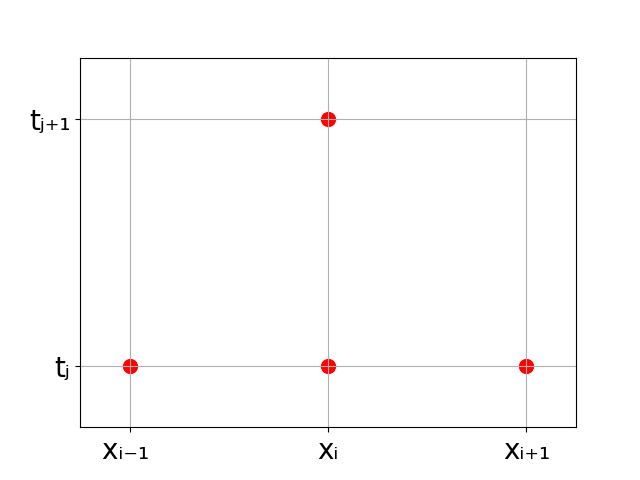
\includegraphics[scale=0.5]{./Imagenes/Bitmap/1dheat.png}
	\caption{Representación en la malla del esquema \ref{eq:1dheat_formula}}
\end{figure}

Para estudiar la convergencia de \ref{eq:1dheat_formula}, primero estudiaremos el siguiente lema:

\begin{lema}
	Suponiendo que $u$ es suficientemente diferenciable, se tiene que
	\begin{equation}
		\label{eq:lema1_eq1}
		u_t(x,t)-u_{x,\bar{x}}(x,t) = \tau(x,t)
	\end{equation}
	donde $t$ es el error de truncamiento, definido como
	\begin{equation}
		\label{eq:lema1_eq2}
		\tau(x,t) = \frac{\Delta t}{2}\frac{\partial^2 u}{\partial t^2} + \frac{\Delta x^2}{12}\frac{\partial^4u}{\partial x^4} + \xi_{\Delta x, \Delta t}.
	\end{equation}
	Siendo $\xi_{\Delta x, \Delta t}$ un número real que cumple que
	\begin{equation*}
		\xi_{\Delta x, \Delta t} \xrightarrow[\Delta x \rightarrow 0, \Delta t\rightarrow 0]{} 0 
	\end{equation*}
	
\end{lema}

\begin{proof}
	Haciendo el desarrollo de Taylor de orden 2 para la función $u$ con centro en el punto $(x,t)$ tenemos
	\begin{equation*}
		\begin{split}
		u(x,t+\Delta t)=u(x,t) + \frac{\partial u}{\partial t}\Delta t + \frac{1}{2}\frac{\partial^2u}{\partial t^2}\Delta t^2 + \xi^1_{\Delta x, \Delta t}\Delta t^2 \Rightarrow \\
		u_t(x,t) - \frac{\partial u}{\partial t} = \frac{\Delta t^2}{2}\frac{\partial^2u}{\partial t^2}\Delta t + \xi_{\Delta x, \Delta t}^1\Delta t
		\end{split}
	\end{equation*}
	Siendo $\xi^1$ un número con las mismas propiedades que $\xi$.
	Despejando la última ecuación, obtenemos el primer sumando de \ref{eq:lema1_eq1}, así como el de la ecuación \ref{eq:lema1_eq2}, y nos sobra $- \frac{\partial u}{\partial t}$ a la izquierda y $\xi_{\Delta x, \Delta t}^1\Delta t$ a la derecha.
	
	Si ahora hacemos los desarrollos de Taylor de orden 4 para la misma función pero en otros puntos, obtenemos
	\begin{equation*}
		u(x+\Delta x,t)=u(x,t)+\frac{\partial u}{\partial x}\Delta x+\frac{1}{2!}\frac{\partial^2 u}{\partial x^2}\Delta x^2 + \frac{1}{3!}\frac{\partial^3u}{\partial x^3}\Delta x^3+\frac{1}{4!}\frac{\partial^4u}{\partial x^4}\Delta x^4 + \xi_{\Delta x, \Delta t}^2\Delta x^4
	\end{equation*}
	y
	\begin{equation*}
		u(x-\Delta x,t)=u(x,t)-\frac{\partial u}{\partial x}\Delta x+\frac{1}{2!}\frac{\partial^2 u}{\partial x^2}\Delta x^2 - \frac{1}{3!}\frac{\partial^3u}{\partial x^3}\Delta x^3+\frac{1}{4!}\frac{\partial^4u}{\partial x^4}\Delta x^4 + \xi_{\Delta x, \Delta t}^3\Delta x^4
	\end{equation*}
	Siendo $\xi_{\Delta x, \Delta t}^2$ y $\xi_{\Delta x, \Delta t}^3$ números que cumplen las mismas propiedades que $\xi$.
	Ahora, si sumamos las dos últimas ecuaciones, ya que se nos cancelan los términos con exponente impar, obtenemos
	\begin{equation*}
		u_{x,\bar{x}} - \frac{\partial^2u}{\partial x^2}=\frac{1}{12}\frac{\partial^2u}{\partial x}\Delta x^2 + (\xi_{\Delta x, \Delta t}^2+\xi_{\Delta x, \Delta t}^3)\Delta x^2
	\end{equation*}

	Si restamos todo, tendiendo en cuenta que $\frac{\partial u}{\partial t} - \frac{\partial^2u}{\partial x^2}=0$, obtenemos precisamente la igualdad \ref{eq:lema1_eq1}, siendo $\xi_{\Delta x, \Delta t} = \xi_{\Delta x, \Delta t}^1\Delta t - (\xi_{\Delta x, \Delta t}^2+\xi_{\Delta x, \Delta t}^3)\Delta x^2$, por lo que se confirma que tiende a 0 cuando los incrementos tienden a 0.
\end{proof}

\begin{teorema}
	Si $0<\lambda<\frac{1}{2}$, el método numérico \ref{eq:1dheat_formula} es convergente, o dicho de otra forma, si $\epsilon_{i,j}$ es el error de aproximación del método, $\sup_{i,j}\epsilon(i,j)\rightarrow0$ si $\Delta t, \Delta x \rightarrow 0$ y el error inicial tiende a 0.
\end{teorema}



\begin{proof}
	Teniendo en cuenta el lema anterior, si ahora repetimos las cuentas de \ref{eq:principio_aprox} obtendríamos \ref{eq:1dheat_formula} pero añadiendo el sumando $\Delta t\tau_{i,j}$, por lo que cada vez que utilizamos esa fórmula estamos añadiendo ese error. Por ello, podemos deducir que
	\begin{equation*}
		\epsilon_{i,j+1} = (1-2\lambda)\epsilon_{i,j}+\lambda(\epsilon_{i+1,j}+\epsilon_{i-1,j})+ \Delta t\tau_{i,j}
	\end{equation*}
	Ahora, si definimos
	\begin{equation*}
		E_j=\sup_{i}|\epsilon_{i,j}|\hspace{30px}\tau=\sup_{i,j}|\tau_{i,j}|
	\end{equation*}
	tenemos que
	\begin{equation*}
		E_j+1\leq E_j+\Delta t\tau
	\end{equation*}
	por tanto, mediante una inducción trivial tenemos que
	\begin{equation*}
		E_j \leq E_0 + j\Delta t\tau = E_0+t_j\tau\hspace{15px}\forall j\geq0
	\end{equation*}
	
	Con esto ya tenemos el resultado, pues está claro, por su definición, que $\tau$ tiende a 0 cuando $\Delta t, \Delta x$ tienden a 0, luego el error está acotado por algo que tiende a 0, lo que implica que tiende a 0.
\end{proof}

\section{Caso bidimensional}

En el caso bidimensional, la ecuación que tenemos será
\begin{equation}\label{eq:2dheat}
	\frac{\partial u}{\partial t}=\frac{\partial^2u}{\partial x^2}+\frac{\partial^2u}{\partial y^2}
\end{equation}

\com{Voy a dejar esto en stand by, estoy teniendo problemas para encontrar algún teorema de existencia y unicidad para alguna condición inicial, y por tanto no sé que condiciones iniciales voy a acabar pidiéndole.}




